\documentclass{standalone}
\usepackage{tikz}
\usetikzlibrary{patterns, positioning}
\usepackage[sfdefault]{ClearSans} %% option 'sfdefault' activates Clear Sans as the default text font
\usepackage[T1]{fontenc}

\begin{document}
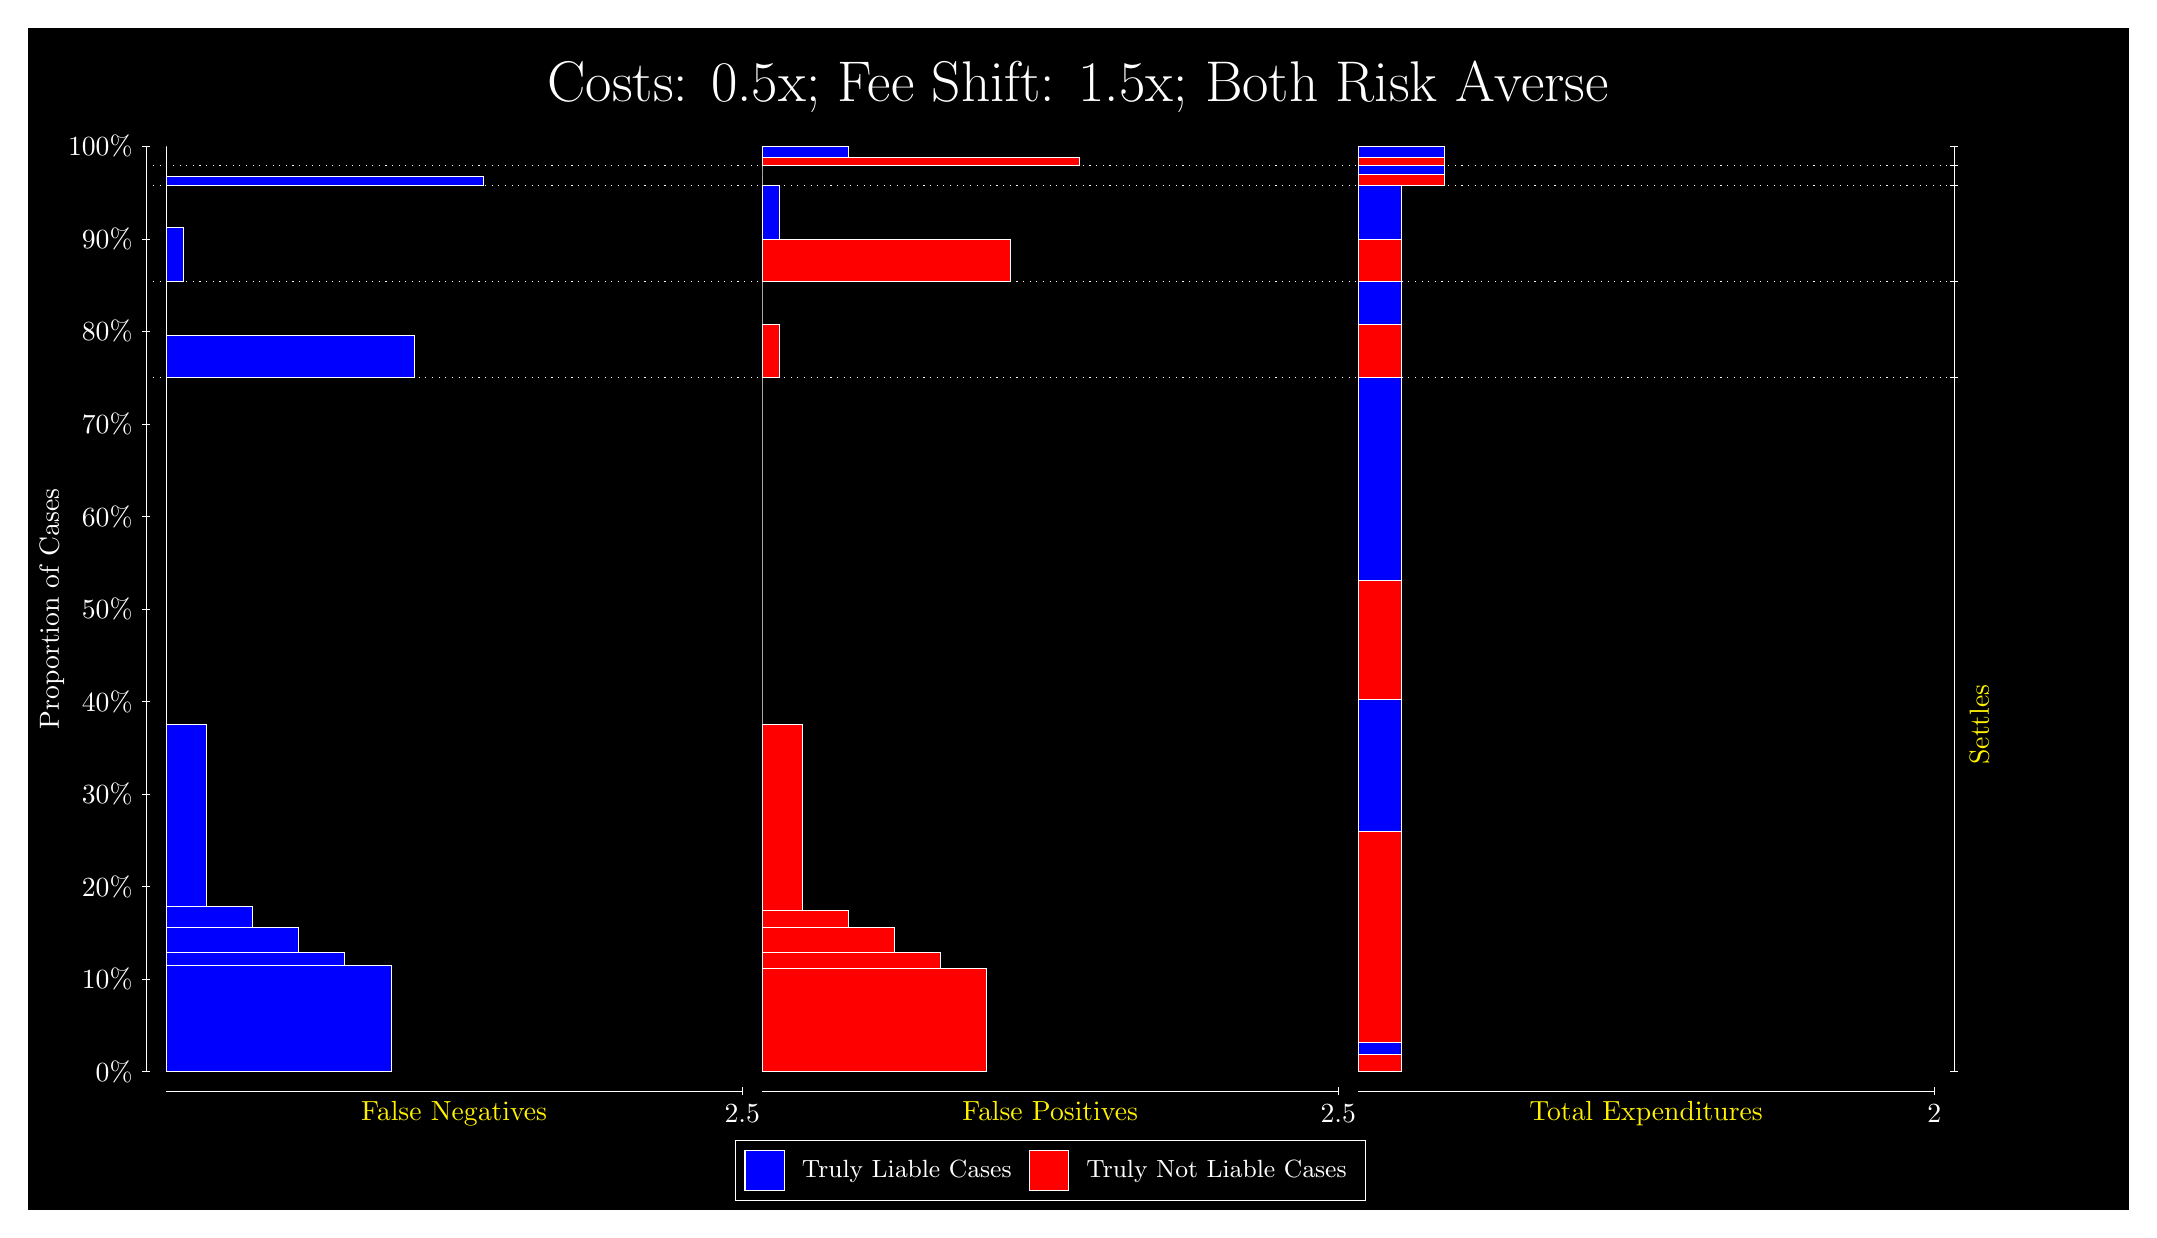
\begin{tikzpicture}
\draw[fill=black] (0,0) rectangle (26.667,15);
\draw[text=white] (0,13.5) rectangle (26.667,15) node[midway] {\huge Costs: 0.5x; Fee Shift: 1.5x; Both Risk Averse};
\draw[white, very thin] (1.5,1.75) -- (1.5,13.5);
\node[rotate=90, text=white, anchor=center] at (0.3, 7.625) {Proportion of Cases};
\draw[white, very thin] (1.45,1.75) -- (1.55,1.75);
\node[text=white, anchor=east] at (1.45, 1.75) {0\%};
\draw[white, very thin] (1.45,2.925) -- (1.55,2.925);
\node[text=white, anchor=east] at (1.45, 2.925) {10\%};
\draw[white, very thin] (1.45,4.1) -- (1.55,4.1);
\node[text=white, anchor=east] at (1.45, 4.1) {20\%};
\draw[white, very thin] (1.45,5.275) -- (1.55,5.275);
\node[text=white, anchor=east] at (1.45, 5.275) {30\%};
\draw[white, very thin] (1.45,6.45) -- (1.55,6.45);
\node[text=white, anchor=east] at (1.45, 6.45) {40\%};
\draw[white, very thin] (1.45,7.625) -- (1.55,7.625);
\node[text=white, anchor=east] at (1.45, 7.625) {50\%};
\draw[white, very thin] (1.45,8.8) -- (1.55,8.8);
\node[text=white, anchor=east] at (1.45, 8.8) {60\%};
\draw[white, very thin] (1.45,9.975) -- (1.55,9.975);
\node[text=white, anchor=east] at (1.45, 9.975) {70\%};
\draw[white, very thin] (1.45,11.15) -- (1.55,11.15);
\node[text=white, anchor=east] at (1.45, 11.15) {80\%};
\draw[white, very thin] (1.45,12.325) -- (1.55,12.325);
\node[text=white, anchor=east] at (1.45, 12.325) {90\%};
\draw[white, very thin] (1.45,13.5) -- (1.55,13.5);
\node[text=white, anchor=east] at (1.45, 13.5) {100\%};

\draw[white, very thin] (24.457,1.75) -- (24.457,13.5);
\draw[white, very thin] (24.407,1.75) -- (24.507,1.75);
\node[anchor=west] at (24.407, 1.75) {};
\draw[white, very thin] (24.407,10.564) -- (24.507,10.564);
\node[anchor=west] at (24.407, 10.564) {};
\draw[white, very thin] (24.407,11.784) -- (24.507,11.784);
\node[anchor=west] at (24.407, 11.784) {};
\draw[white, very thin] (24.407,13.005) -- (24.507,13.005);
\node[anchor=west] at (24.407, 13.005) {};
\draw[white, very thin] (24.407,13.253) -- (24.507,13.253);
\node[anchor=west] at (24.407, 13.253) {};
\draw[white, very thin] (24.407,13.5) -- (24.507,13.5);
\node[anchor=west] at (24.407, 13.5) {};

\draw[white, very thin, fill=blue] (1.75,1.75) rectangle (4.6044,3.1047);
\draw[white, very thin, fill=blue] (1.75,3.1047) rectangle (4.0188,3.2625);
\draw[white, very thin, fill=blue] (1.75,3.2625) rectangle (3.4333,3.5824);
\draw[white, very thin, fill=blue] (1.75,3.5824) rectangle (2.8478,3.8507);
\draw[white, very thin, fill=blue] (1.75,3.8507) rectangle (2.2623,6.1568);
\draw[white, very thin, fill=red] (1.75,6.1568) rectangle (1.75,10.564);
\draw[white, very thin, fill=blue] (1.75,10.564) rectangle (4.8971,11.103);
\draw[white, very thin, fill=red] (1.75,11.103) rectangle (1.75,11.784);
\draw[white, very thin, fill=blue] (1.75,11.784) rectangle (1.9696,12.466);
\draw[white, very thin, fill=red] (1.75,12.466) rectangle (1.75,13.005);
\draw[white, very thin, fill=blue] (1.75,13.005) rectangle (5.7754,13.118);
\draw[white, very thin, fill=red] (1.75,13.118) rectangle (1.75,13.253);
\draw[white, very thin, fill=red] (1.75,13.253) rectangle (1.75,13.365);
\draw[white, very thin, fill=blue] (1.75,13.365) rectangle (1.75,13.5);
\draw[white, very thin, fill=red] (9.3189,1.75) rectangle (12.173,3.0652);
\draw[white, very thin, fill=red] (9.3189,3.0652) rectangle (11.588,3.2624);
\draw[white, very thin, fill=red] (9.3189,3.2624) rectangle (11.002,3.5823);
\draw[white, very thin, fill=red] (9.3189,3.5823) rectangle (10.417,3.797);
\draw[white, very thin, fill=red] (9.3189,3.797) rectangle (9.8312,6.1568);
\draw[white, very thin, fill=blue] (9.3189,6.1568) rectangle (9.3189,10.564);
\draw[white, very thin, fill=red] (9.3189,10.564) rectangle (9.5384,11.245);
\draw[white, very thin, fill=blue] (9.3189,11.245) rectangle (9.3189,11.784);
\draw[white, very thin, fill=red] (9.3189,11.784) rectangle (12.466,12.324);
\draw[white, very thin, fill=blue] (9.3189,12.324) rectangle (9.5384,13.005);
\draw[white, very thin, fill=red] (9.3189,13.005) rectangle (9.3189,13.14);
\draw[white, very thin, fill=blue] (9.3189,13.14) rectangle (9.3189,13.253);
\draw[white, very thin, fill=red] (9.3189,13.253) rectangle (13.344,13.365);
\draw[white, very thin, fill=blue] (9.3189,13.365) rectangle (10.417,13.5);
\draw[white, very thin, fill=red] (16.888,1.75) rectangle (17.437,1.9646);
\draw[white, very thin, fill=blue] (16.888,1.9646) rectangle (17.437,2.1224);
\draw[white, very thin, fill=red] (16.888,2.1224) rectangle (17.437,4.8022);
\draw[white, very thin, fill=blue] (16.888,4.8022) rectangle (17.437,6.4768);
\draw[white, very thin, fill=red] (16.888,6.4768) rectangle (17.437,7.9892);
\draw[white, very thin, fill=blue] (16.888,7.9892) rectangle (17.437,10.564);
\draw[white, very thin, fill=red] (16.888,10.564) rectangle (17.437,11.245);
\draw[white, very thin, fill=blue] (16.888,11.245) rectangle (17.437,11.784);
\draw[white, very thin, fill=red] (16.888,11.784) rectangle (17.437,12.324);
\draw[white, very thin, fill=blue] (16.888,12.324) rectangle (17.437,13.005);
\draw[white, very thin, fill=red] (16.888,13.005) rectangle (17.986,13.14);
\draw[white, very thin, fill=blue] (16.888,13.14) rectangle (17.986,13.253);
\draw[white, very thin, fill=red] (16.888,13.253) rectangle (17.986,13.365);
\draw[white, very thin, fill=blue] (16.888,13.365) rectangle (17.986,13.5);
\draw[white, dotted] (1.5,10.564) -- (24.457,10.564);
\draw[white, dotted] (1.5,11.784) -- (24.457,11.784);
\draw[white, dotted] (1.5,13.005) -- (24.457,13.005);
\draw[white, dotted] (1.5,13.253) -- (24.457,13.253);
\draw[white, very thin] (1.75,1.5) -- (9.0689,1.5);
\node[text=yellow, anchor=north] at (5.4094, 1.5) {False Negatives};
\draw[white, very thin] (9.0689,1.45) -- (9.0689,1.55);
\node[text=white, anchor=north] at (9.0689, 1.45) {2.5};

\draw[white, very thin] (9.3189,1.5) -- (16.638,1.5);
\node[text=yellow, anchor=north] at (12.978, 1.5) {False Positives};
\draw[white, very thin] (16.638,1.45) -- (16.638,1.55);
\node[text=white, anchor=north] at (16.638, 1.45) {2.5};

\draw[white, very thin] (16.888,1.5) -- (24.207,1.5);
\node[text=yellow, anchor=north] at (20.547, 1.5) {Total Expenditures};
\draw[white, very thin] (24.207,1.45) -- (24.207,1.55);
\node[text=white, anchor=north] at (24.207, 1.45) {2};

\node[text=yellow, centered, rotate=90] at (24.777, 6.1568) {Settles};





\draw (12.978300999999998,1.5) node[draw=none] (baseCoordinate) {};
\begin{scope}[align=center]
        \matrix[scale=0.5, draw=white, below=0.5cm of baseCoordinate, nodes={draw}, column sep=0.1cm]{
            \node[rectangle, draw, minimum width=0.5cm, minimum height=0.5cm, fill=blue] {}; &
            \node[draw=none, font=\small, text=white] (B) {Truly Liable Cases}; &
            \node[rectangle, draw, minimum width=0.5cm, minimum height=0.5cm, fill=red] {}; &
            \node[draw=none, font=\small, text=white] (B) {Truly Not Liable Cases}; \\
            };
\end{scope}

\end{tikzpicture}
\end{document}